% //////////////////////////////////////// %
% /// Architecture web et relationnel //// %
\section{Architecture web et relationnel}
	%% Architecture classique
	\subsection{Architecture classique}
	\begin{frame}
		\frametitle{Architecture classique}

		\begin{figure}[htb]
			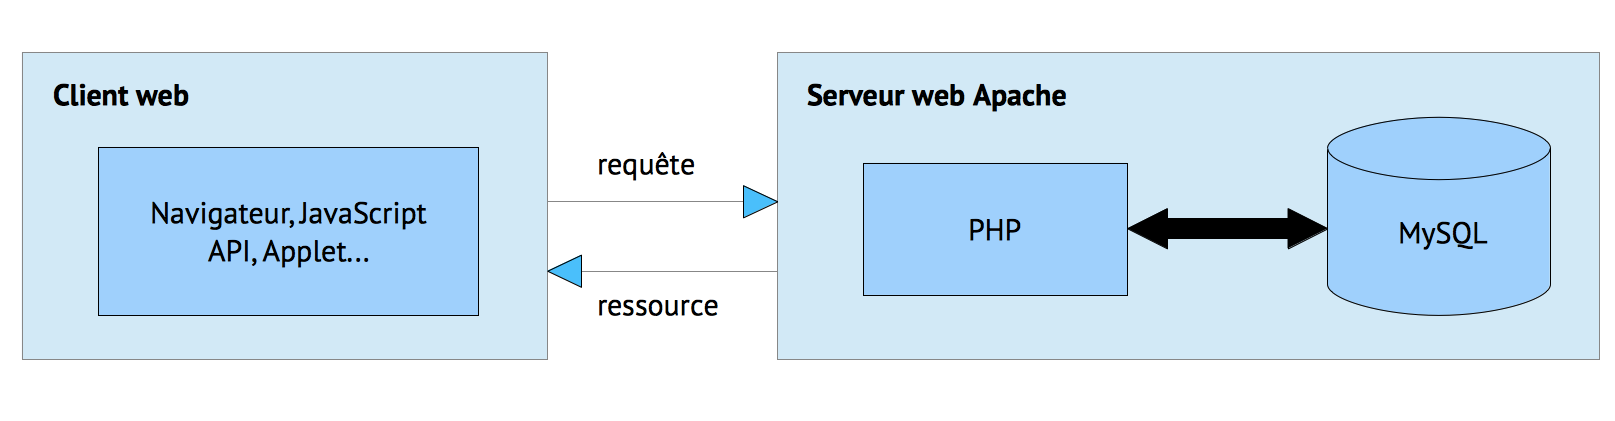
\includegraphics[width=1\textwidth]{images/LAMP.png}
			\caption{La stack LAMP.}
		\end{figure}

		\textbf{Stacks habituelles :}
		\begin{itemize}
			\item LAMP : Linux, Apache, MySQL, PHP — la plus commune ;
			\item LEMP : Linux, Nginx, MySQL, PHP-FPM — commence à remplacer LAMP ;
			\item MEAN : MySQL, Express, AngularJS, Node.js — pour du JavaScript côté serveur.
		\end{itemize}

	\end{frame}

	%% Bilan architecture classique
	\subsection{Bilan architecture classique}
	\begin{frame}
		\frametitle{Bilan architecture classique}

		\textbf{Avantages :}
		\begin{itemize}
			\item Rapide à mettre en place (installation en un clic généralement) ;
			\item Optimisation possible, verticalement le plus souvent ;
		\end{itemize}

		\vspace{20px}

		\textbf{Inconvénients :}
		\begin{itemize}
			\item Il faut une expertise base de données.
		\end{itemize}

	\end{frame}

	%% Qu'est-ce qu'un ORM ?
	\subsection{Qu'est-ce qu'un ORM ?}
	\begin{frame}
		\frametitle{Qu'est-ce qu'un ORM ?}

		\begin{block}{Définition : ORM}
			L'\textbf{O}bject-\textbf{R}elationnal \textbf{M}apping est une technique qui simule une base de données orientée objet à partir d'une base de données relationnelle.
		\end{block}

		\vspace{2px}

		\begin{itemize}
			\item Fait la liaison entre le monde relationnel dans la couche stockage et le monde objet dans l'application ;
			\item Facilité de développement : \textit{pas besoin} d'une connaissance poussée du SQL ;
			\item Facilite les interactions avec la base de données pour les développeurs.
		\end{itemize}

		\vspace{2px}

		\begin{alertblock}{Les limites des ORM}
			Toujours \textbf{beaucoup} moins performant que des requêtes SQL optimisées.
		\end{alertblock}

	\end{frame}

	\begin{frame}
		\frametitle{ORM : exemple de requêtes}

		\begin{listing}[H]
			\inputminted[fontsize=\tiny, linenos=true]{php}{code/eloquent.php}
			\caption{Quelques requêtes basiques avec l'ORM Eloquent (PHP).}
		\end{listing}

		\scriptsize{D'autres ORM : Hibernate (Java), SQLAlchemy (Python), Mongoose (Node.js)\dots}

	\end{frame}